\chapter{4-hydroxymethylpyridine complexes}
\section{\ce{[Cu(N_3)_2(4-hydroxymethylpyridine)]_n}}
\subsection{Synthesis}
0.48 g \ce{Cu(NO_3)_2*3 H_2O} (2 mmol), 0.26 g sodium azide (4 mmol) and 0.22 g 4-(hydroxymethyl)pyridine (2 mmol) were added to 40 mL distilled water. The solution was heated up for 120 minutes at 70$^\circ$C. After filtration the solution was heated up 50 minutes at 70$^\circ$C and then cooled down to RT. Green needles were obtained after one day.\\
 Anal. Calculated for \ce{C_{6}H_{7}CuN_{7}O} (256.74 g/mol): 28.07\% C; 2.75\% H; 38.19\% N;\\
Found: 28.09 \% C; 2.78\% H; 38.09 \% N;\\
IR (ATR, cm$^{-1}$): 3355 (w),  2025 (vs), 1616 (m), 1562 (w), 1505 (w), 1432 (m), 1289 (m), 1221 (m), 1034 (s), 960 (w), 806 (m), 618 (m), 587 (m), 483 (m)

\newpage
\begin{figure}[htpb!]
\centering
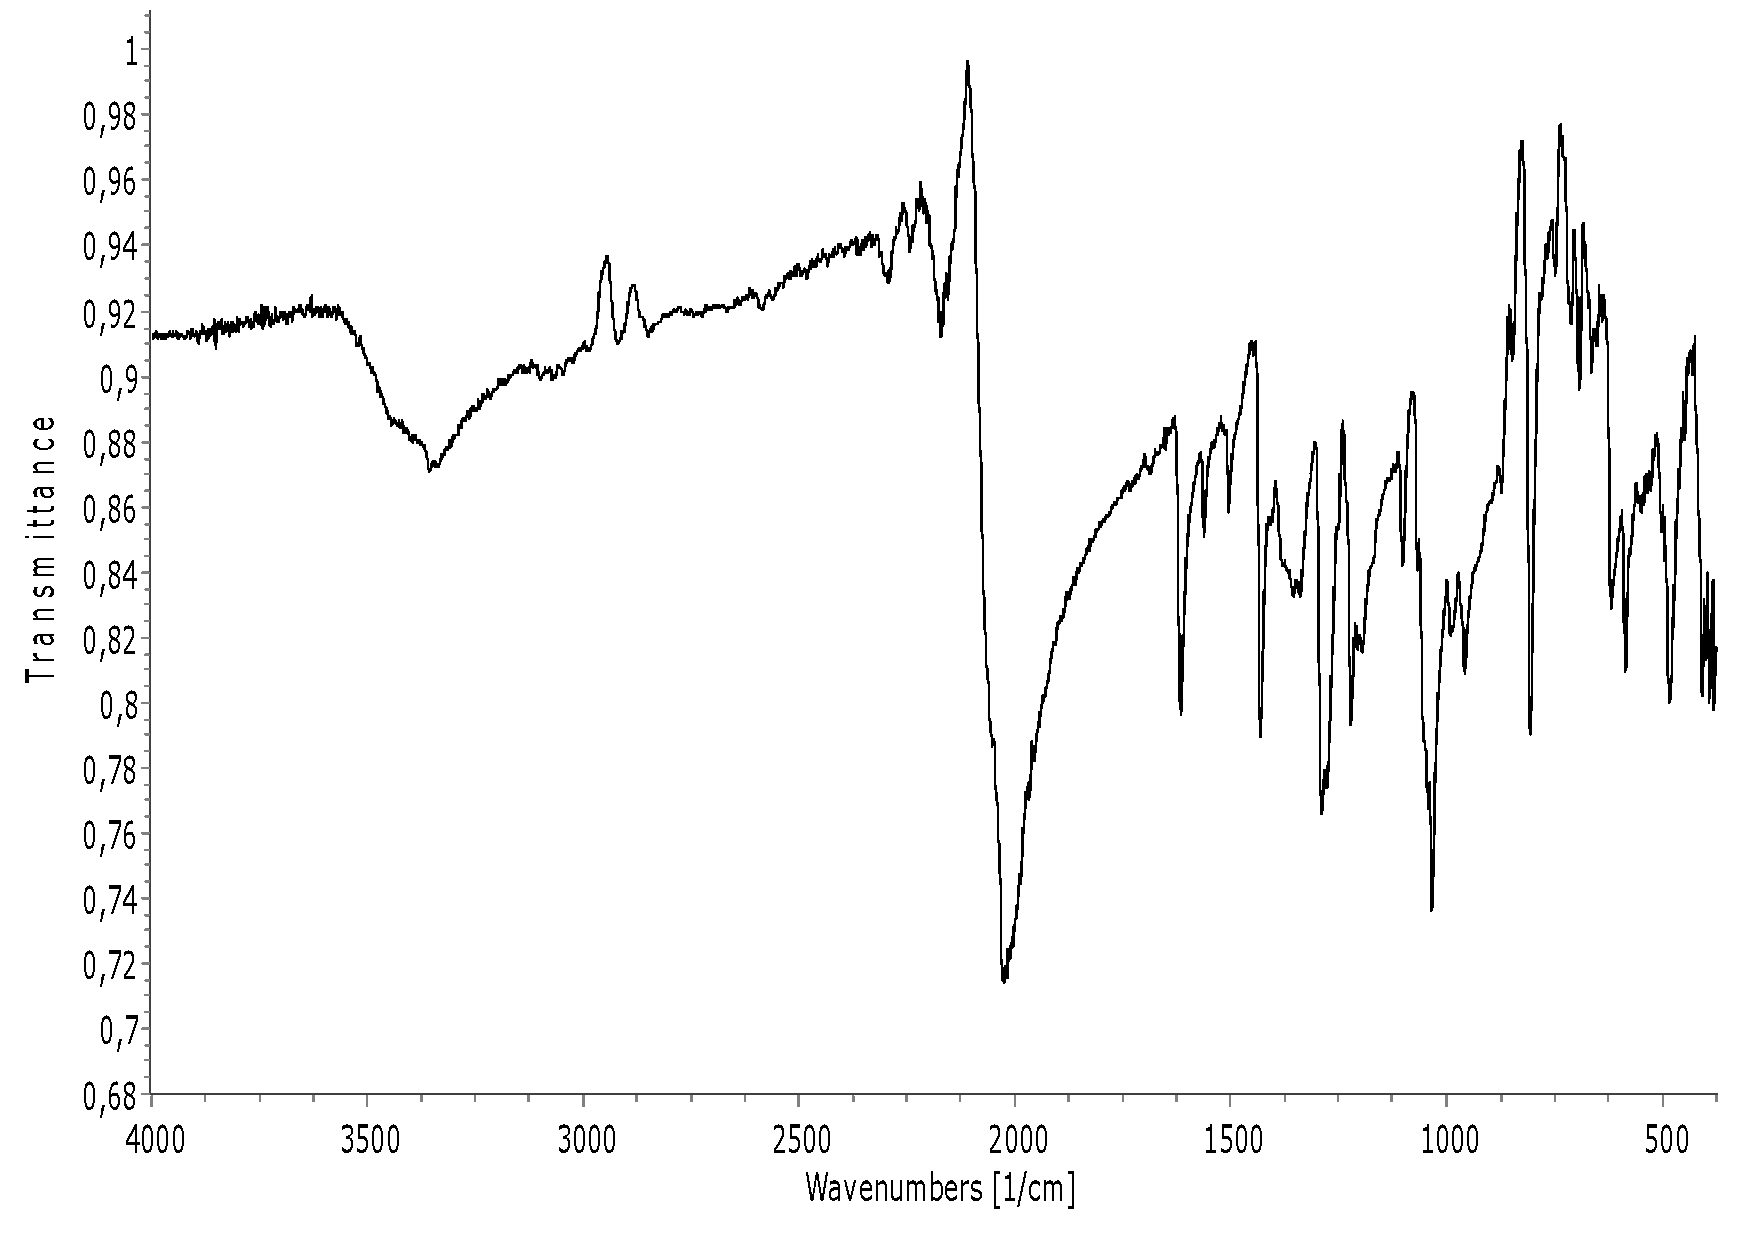
\includegraphics[width=1\textwidth]{figures/CuA4HOMP-IR.pdf}
\caption{IR-Spectrum of \ce{[Cu(N_3)_2(4-HOMepy)]_n}}
\end{figure}

\subsection{Structural characterization}
 Selected bond parameters of \ce{[Cu(N_3)_2(4-HOMepy)]_n} are summarized in table \ref{batab:CuA4HOMP}, a perspective view of a section of the polymeric chain is given in fig. \ref{fig:CuA4HOMP_pv} and a packing view in fig. \ref{fig:CuA4HOMP_packv}. The Cu(1) metal center is penta-coordinated by pyridine N donor atom of a 4-hydroxymethylpyridine molecule and four N atoms of azide groups. The \ce{CuN5} chromophore forms a distorted square pyramid (SP) with a $\tau$-value of 0.24 ($\tau$-values of 1 and 0 refer to ideal geometries of trigonal bipyramid (TBP) and square pyramid (SP), respectively) \cite{addison}. The apical site is occupied by N(23b) [Cu(1)-N(23b) = 2.462(2) \AA]. The basal Cu-N bond distances range from 1.972(2) to 2.005(2) \AA. The azide groups behave differently. Azide groups N(11)-N(12)-N(13) and N(11a)-N(12a)-N(13a) act as di-EO bridges to connect the polyhedra of Cu(1) and Cu(1a) to centrosymmetric dimeric subunits. The bond parameters within their four-membered \ce{Cu2N2} rings are: Cu(1)-N(11)-Cu(1a) = 101.82(10), N(11)-Cu(1)-N(11a) = 78.18(10), Cu(1)-N(11)-N(12) =  128.59(18) and Cu(1a)-N(11)-N(12) = 125.00(18)$^\circ$. The azide group N(21)-N(22)-N(23) act as asymmetrical single EE azido bridge, with N(21) ligated in basal position and N(23) ligated in axial position. Four such single EE azide bridges connect the centrosymmetric dimeric Cu(1)..Cu(1a) subunits to generate double chains of polyhedra oriented along the a-axis of the unit cell. The Cu(1)-N(21)-Cu(1c)-N(23)-N(22) bond angles are 123.98(19) and 110.51(18)$^\circ$, respectively, and the Cu(1)-N(21)..N(23)-Cu(1c) torsion angle is -92.3$^\circ$. The intra-chain Cu(1)..Cu(1a) and Cu(1)..Cu(1c) distances are 3.1042(6) and 5.2153(9) \AA, and the shortest inter-chain metal-metal separation is 7.5484(12) \AA. The bond distances and bond angle of the EO azide bridge are 1.220(3) \AA, 1.139(4) \AA, and 177.8(3)$^\circ$, whereas the corresponding bond parameters for the EE azide bridge are 1.199(3) \AA, 1.161(3) \AA, and 176.9(3)$^\circ$. The 4-hydroxypyridine molecule forms hydrogen bond of  the type O-H\ce{***}N (O(17)-H(91)\ce{***}N(13’)  = 144(6)$^\circ$, O(17)\ce{***}N(13’) = 2.990(6) \AA; symmetry code (‘): 1-x,2-y,1-z).



\renewcommand{\arraystretch}{1.2}
\begin{table}[htpb!]
\centering
\captionabove{Selected bond lengths (\AA) and angles ($^\circ$) for \ce{[Cu(N_3)_2(4-HOMepy)]_n}. Symmetry codes: (a) 2-x, 1-y, 1-z; (b) -1+x, y, z; (c) 2-x, 1-y, 1-z; (d) 1+x, y, z; (e) -x, 1-y, 1-z; (g) -2x, y, z. }
\begin{tabular}{|l|l|l|l|}
\hline
Cu(1)-N(11a) & 2.005(2) & Cu(1)-N(23b) & 2.462(2)\\
\hline
Cu(1)-N(1) & 1.981(2) & Cu(1)-N(11) & 1.995(2)\\
\hline
Cu(1)-N(21) & 1.972(2) & N(11)-N(12) & 1.220(3)\\
\hline
N(12)-N(13) & 1.139(4) & N(21)-N(22) & 1.199(3)\\
\hline
N(22)-N(23) & 1.161(3) &  & \\
\hline
\hline
N(21)-Cu(1)-N(1) & 94.55(9) & N(21)-Cu(1)-N(11) & 159.74(10)\\
\hline
N(11)-Cu(1)-N(1) & 96.01(9) & N(21)-Cu(1)-N(11a) & 91.04(9)\\
\hline
N(11)-Cu(1)-N(11a) & 78.18(10) & N(21)-Cu(1)-N(23b) & 103.39(9)\\
\hline
N(1)-Cu(1)-N(23b) & 93.42(9) & N(11)-Cu(1)-N(23b) & 93.19(9)\\
\hline
N(11a)Cu(1)-N(23b) & 86.84(9) & N(1)-Cu(1)-N(11a) & 174.18(9)\\
\hline
Cu(1)-N(11)-N(12) & 128.5(18) &N(11)-N(12)-N(13) & 177.8(3)\\
\hline
Cu(1)-N(21)-C(22) & 123.98(19) & N(21)-N(22)-N(23) & 176.9(3)\\
\hline
Cu(1a)-N(11)-N(12) & 125.00(18) & Cu(1)-N(11)-Cu(1a) & 101.82(10)\\
\hline
Cu(1c)-N(23)-N(22) & 110.51(18) &  &\\
\hline

\end{tabular}
\label{batab:CuA4HOMP}
\end{table}






\begin{figure}[!htpb]
\centering
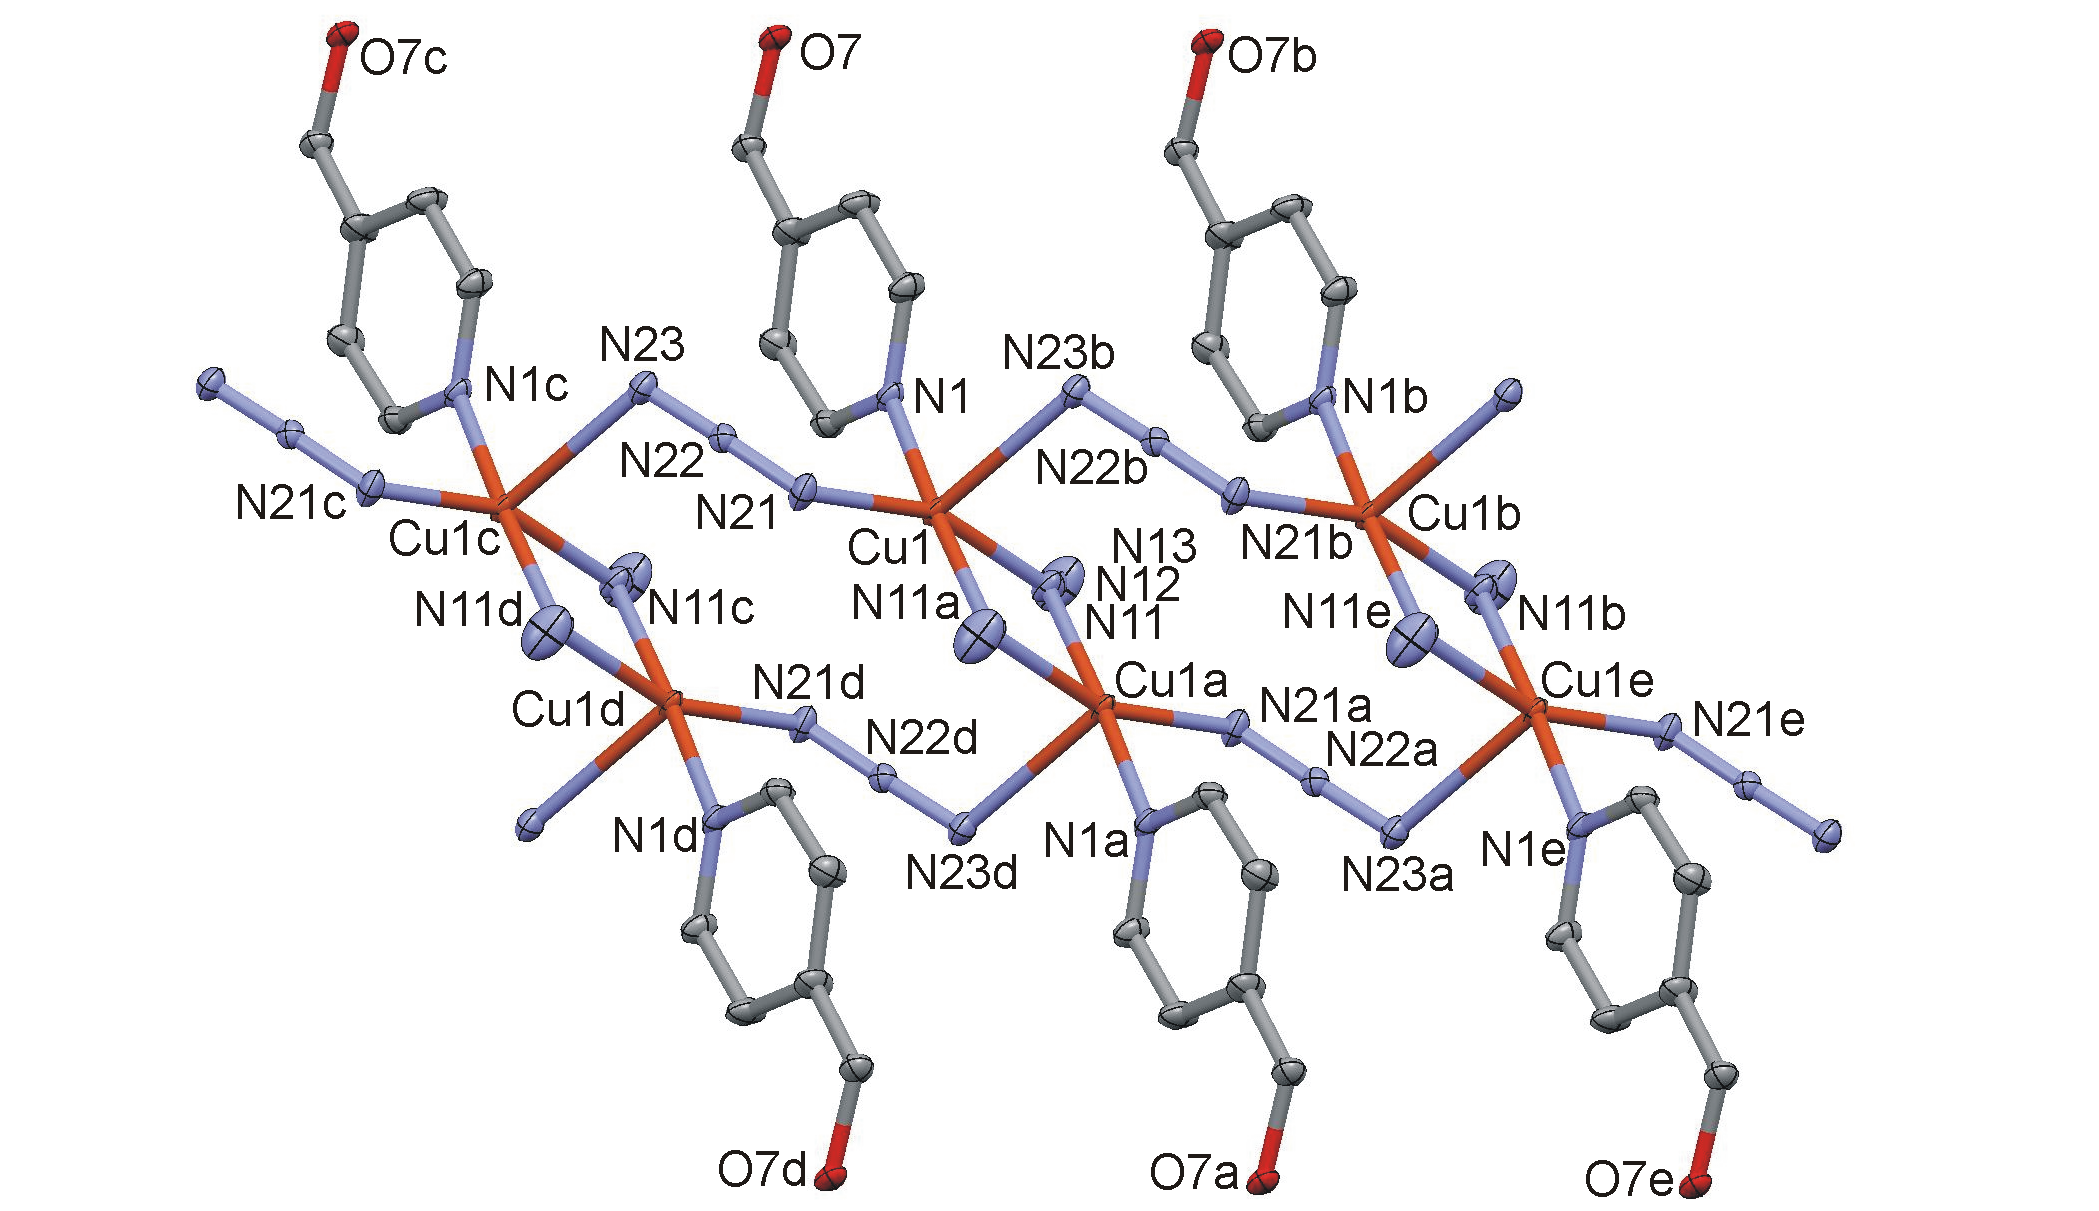
\includegraphics[width=0.90\textwidth]{figures/cuahomp_FIGm12.png}
\caption[Perspective view of \ce{[Cu(N_3)_2(4-HOMepy)]_n}]{Perspective view of a section of the polymeric chain of \ce{[Cu(N_3)_2(4-HOMepy)]_n} with the atom numbering scheme. 
Symmetry codes:(a) 2-x,1-y,1-z; (b) 1+x,y,z; (c) -1+x,y,z; (d) 1-x,1-y,1-z; (e) 3-x,1-y,1-z.}
\label{fig:CuA4HOMP_pv}
\vspace{\floatsep}
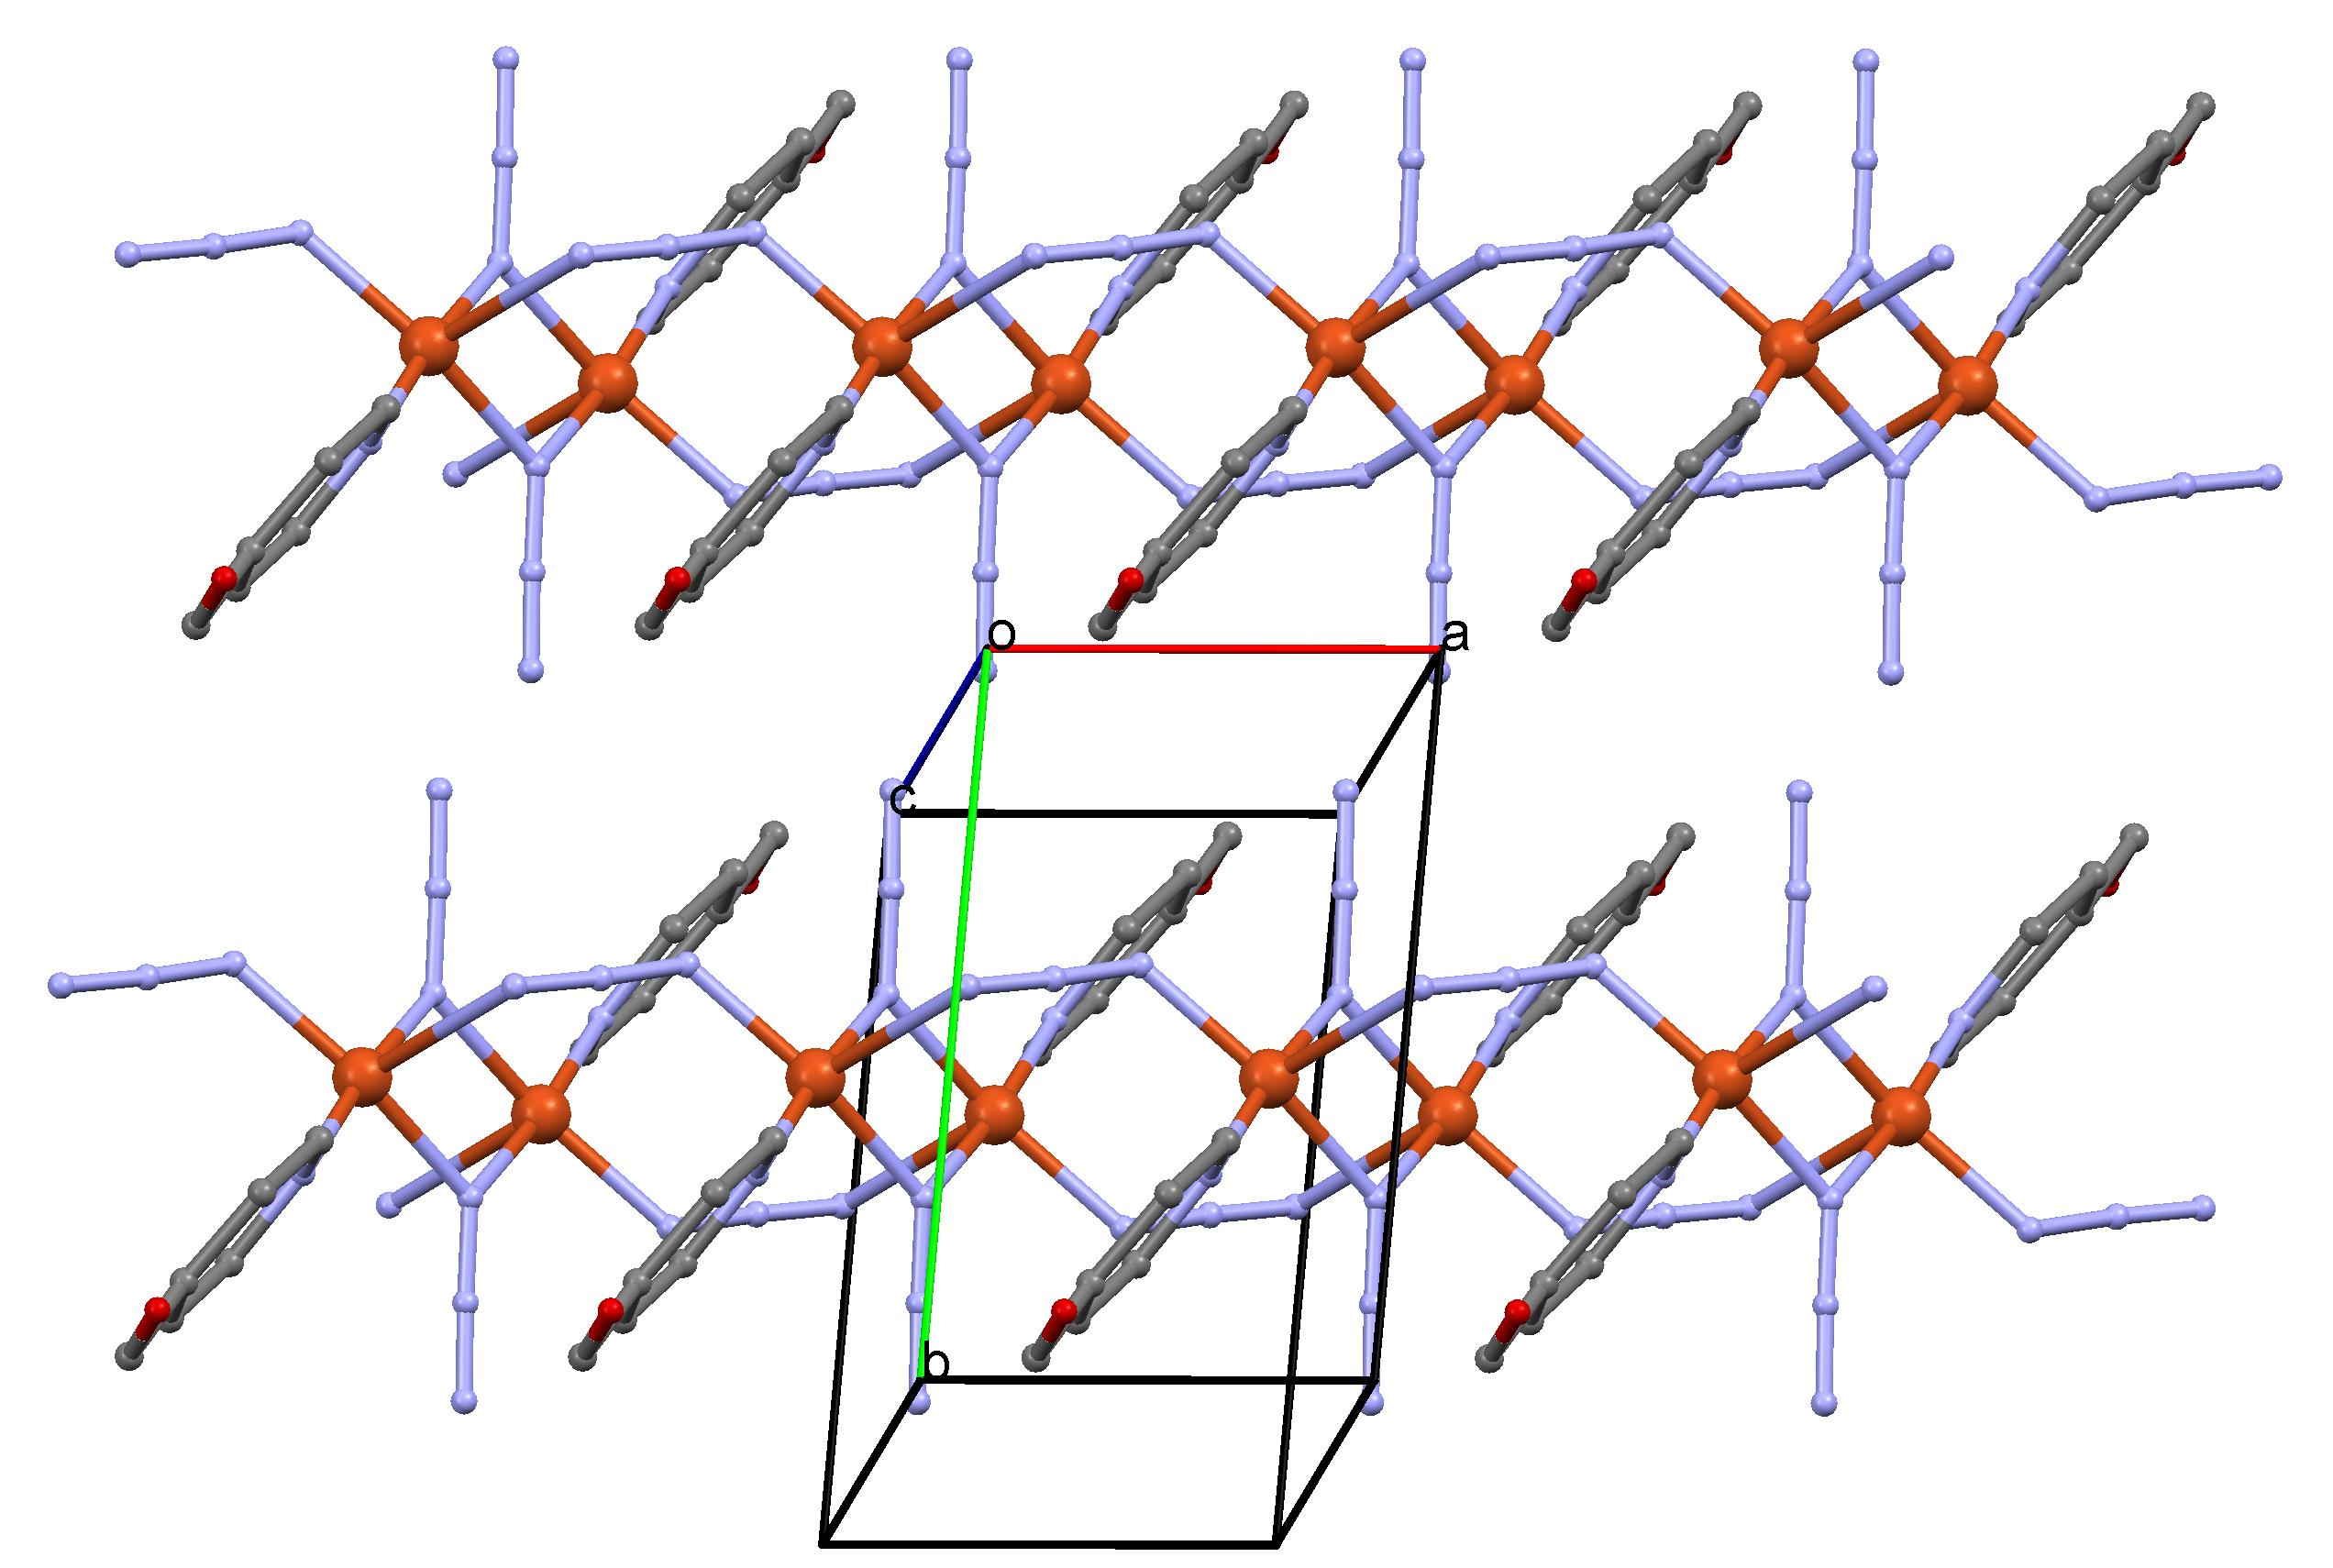
\includegraphics[width=0.90\textwidth]{figures/cuahomp_CC.png}
\caption{Packing plot of \ce{[Cu(N_3)_2(4-HOMepy)]_n}.}
\label{fig:CuA4HOMP_packv}
\end{figure}


\renewcommand{\arraystretch}{1.5}

\begin{table}
\captionabove{Crystallographic data and processing parameter of \ce{[Cu(N_3)_2(4-HOMepy)]_n}}
\centering
\begin{tabular}{ | l |  l | }
\hline
Empirical formula & \ce{C_{6}H_{7}CuN_{7}O}\\
\hline
Formula mass & 256.74\\
\hline
System & triclinic\\
\hline
Space group & P-1\\
\hline
a ({\AA}) & 5.2153(8)\\
\hline
b ({\AA}) & 9.6409(15)\\
\hline
c ({\AA}) & 9.7206(15)\\
\hline
$\alpha$ ($^\circ$) & 106.898(3)\\
\hline
$\beta$ ($^\circ$) & 97.332(3)\\
\hline
$\gamma$ ($^\circ$) & 94.151(3)\\
\hline
V (\AA$^{3}) $  & 460.73(12)\\
\hline
Z & 2\\
\hline
T (K) & 100(2)\\
\hline
$\mu$ (mm$^{-1}$) & 2.354\\
\hline
 D$_{calc}$ (Mg/m$^{3}$) & 1.851\\
\hline
Crystal size (mm) & 0.10 x 0.15 x 0.02\\
\hline
$\theta$ max ($^\circ$) & 29.99\\
\hline
Data collected & 12368\\
\hline
Unique refl./ R$_{int}$ & 2692 / 0.0207\\
\hline
Parameters & 160\\
\hline
Goodness-of-Fit on F$^{2}$ & 1.369\\
\hline
R1 / wR2 (all data) & 0.0313 /0.0878\\
\hline
Residual extrema (e/\AA$^{3}$) & 0.59 /-0.68\\
\hline
\end{tabular}

\label{ptab:CuA4HOMP}

\end{table}



